% Formação de imagem numa lente convergente
% Feito para o ÉguaTeX (eguatex.com.br). Uso livre (CC0 1.0).
%
% Compile e pronto: sai só a figura, em PDF.
% Para pôr no seu trabalho, use o PDF com \includegraphics ou copie
% o bloco tikzpicture para dentro de uma figure.
%
% A posição e o tamanho da imagem saem da equação das lentes delgadas,
% 1/f = 1/p + 1/p', e do aumento A = -p'/p. Use p maior que f
% para a imagem ser real e invertida.
\documentclass[tikz,border=4pt]{standalone}
\usepackage[T1]{fontenc}
\usepackage{lmodern}

\colorlet{corObj}{blue!70!black}
\colorlet{corImg}{red!75!black}
\colorlet{corRaio}{orange!85!black}

\begin{document}
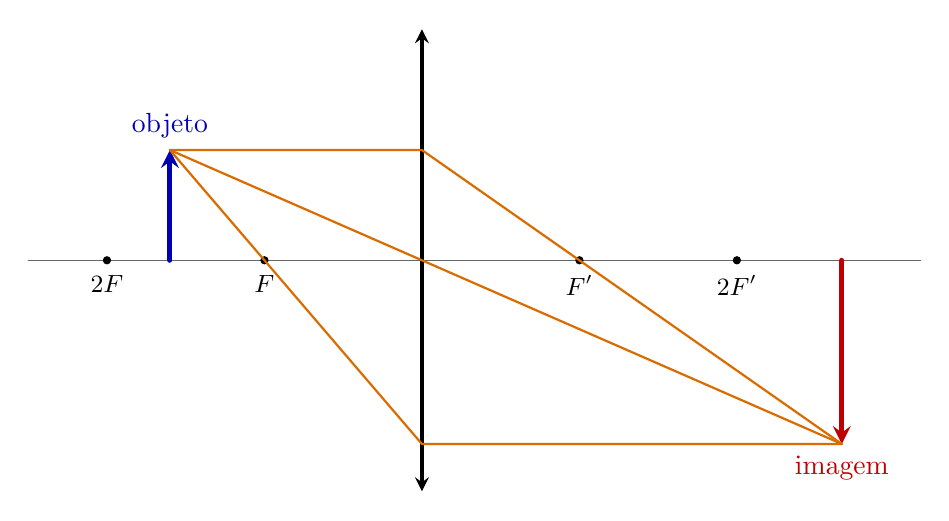
\begin{tikzpicture}[line cap=round, line join=round, >=stealth,
  raio/.style={line width=0.8pt, corRaio},
  seta/.style={->, line width=1.8pt}]

% Mude estes números e o desenho e os rótulos acompanham.
\def\f{2}     % distância focal, em cm
\def\p{3.2}   % distância do objeto até a lente, em cm (maior que f)
\def\h{1.4}   % altura do objeto, em cm

\pgfmathsetmacro{\q}{1/(1/\f-1/\p)}   % distância da imagem
\pgfmathsetmacro{\hi}{-\h*\q/\p}      % altura da imagem (negativa: invertida)
\pgfmathsetmacro{\L}{max(\p,2*\f)+1}  % até onde vai o eixo à esquerda
\pgfmathsetmacro{\Rr}{max(\q,2*\f)+1} % até onde vai o eixo à direita
\pgfmathsetmacro{\H}{max(\h,-\hi)+0.6}

% eixo óptico e lente
\draw[black!60] (-\L,0) -- (\Rr,0);
\draw[<->, line width=1.2pt] (0,-\H) -- (0,\H);
\foreach \x/\n in {-\f/F, \f/F', {-2*\f}/2F, {2*\f}/2F'} {
  \fill (\x,0) circle[radius=1.5pt];
  \node[below=2pt, font=\small] at (\x,0) {$\n$};
}

% objeto e imagem
\draw[seta, corObj] (-\p,0) -- (-\p,\h) node[above] {objeto};
\draw[seta, corImg] (\q,0) -- (\q,\hi) node[below] {imagem};

% raios notáveis
% 1: paralelo ao eixo, depois passa pelo foco F'
\draw[raio] (-\p,\h) -- (0,\h) -- (\q,\hi);
% 2: pelo centro da lente, sem desviar
\draw[raio] (-\p,\h) -- (\q,\hi);
% 3: pelo foco F, depois sai paralelo ao eixo
\draw[raio] (-\p,\h) -- (0,\hi) -- (\q,\hi);
\end{tikzpicture}
\end{document}
